\documentclass{beamer}
\usepackage{tikz}
\usepackage[orientation=landscape,size=a0,scale=2]{beamerposter}
\usepackage[absolute,overlay]{textpos}
\usetikzlibrary{arrows}
\usetikzlibrary{petri}

\begin{document}

\begin{textblock}{15}(0.5, 0.5)
    \begin{block}{}
        \centering
        \Large Suppression of Variation in Cell-Size: A Control Theoretic Approach \\
        \large Dilawar Singh, \texttt{dilawars@ncbs.res.in}
    \end{block}
    \begin{block}{Abstract}

        We propose a  possible mechanism based on control and information theory
        which can be used to control cell size. We explore few network
        topologies of a simple control network which can keep the size of the
        cell at a fixed value while giving a upper bound on the size of the
        Endosome.

\end{block}
\end{textblock}

\begin{textblock}{5}(0.5,3.5)

    \begin{block}{Network under study}
        \begin{figure}
            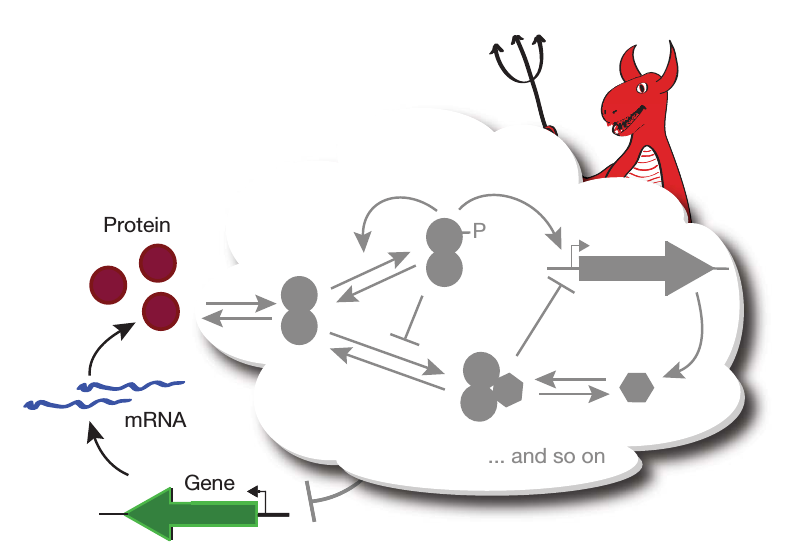
\includegraphics[scale=1]{./fig_mrna_protein.png}
            \begin{tikzpicture}[
                ]
            \node[place,tokens=1,label=above:$X_1$] (X1) at (0,0) {};
            \node[place,colored tokens={red,red,red},label=below:$X_2$] (X2) at (0,-5) {};

            \node[transition,minimum size=10mm,blue,fill,label=above:$f$] (birth) at (3,0) {};
            \node[transition,red,minimum size=10mm,fill,label=below:$\tau$] (death) at (3,-5) {};

            \node[place,label=above:Birth] (Xb) at (10,0) {$+1$};
            \node[place,label=below:Death] (Xd) at (10,-5) {$-1$};


            \draw[ultra thick,-triangle 90] (X1) to (birth) to (Xb);
            \draw[ultra thick,-triangle 90] (X1) to  (death);

            \draw[ultra thick,-triangle 90] (X2) to (death)  to (Xd);
            \draw[ultra thick,-triangle 90] (X2) to (birth);

            \draw[ultra thick,-triangle 90,blue] (Xb) to [bend right]  (birth);
            \draw[ultra thick,-triangle 90,blue] (Xb) to (death);

            \draw[ultra thick,red,-triangle 90] (Xd) to [bend left] (death) (Xd) to (birth);

            \end{tikzpicture}
        \caption{\small On left, mRNA/Protein network. In our scheme $X_1$ is
    mRNA and $X_2$ is its protein. On right, an equivalent Petri net with some
    details omitted. } 

    \label{fig:demon} 
    \end{figure}

    \begin{eqnarray*}
        \tiny
            X_1 \xrightarrow{f(x_2(-\infty,t))} X_1 + 1 \qquad X_1 \xrightarrow{\tau_{x_1}} X_1 -1 \\
            X_2 \xrightarrow{f(x_1)} X_2 + 1 \qquad X_2 \xrightarrow{\tau_{x_2}} X_2 - 1
    \end{eqnarray*}

   
    \end{block}

\end{textblock}

\end{document}
